%  LaTeX support: latex@mdpi.com
\documentclass[notspecified,article,submit,pdftex,moreauthors]{Definitions/mdpi}

\firstpage{1}
\makeatletter
\setcounter{page}{\@firstpage}
\makeatother
\pubvolume{1}
\issuenum{1}
\articlenumber{0}
\pubyear{2026}
\copyrightyear{2026}
\datereceived{}
\daterevised{}
\dateaccepted{}
\datepublished{}

\usepackage{placeins}

\Title{Physics-Guided CNN Detection of Crack-Associated Events from Multiplexed Fiber Bragg Grating Interrogator Signals}

\Author{A.~U{\u g}urveren $^{1,3}$, A.~Gros $^{1}$, E.~Nohutcuo{\u g}lu $^{1,3}$, T.~Teko{\u g}lu $^{1,3}$, K.~Y\"uksel $^{3}$, K.~Chah $^{1}$ and C.~Caucheteur $^{1,2,*}$}
\AuthorNames{A. U{\u g}urveren, A. Gros, E. Nohutcuo{\u g}lu, T. Teko{\u g}lu, K. Y\"uksel, K. Chah and C. Caucheteur}

\address{%
$^{1}$ \quad Electromagnetism and Telecommunication Department, UMONS, 7000 Mons, Belgium;\\
$^{2}$ \quad WEL Research Institute, Avenue Pasteur 6, 1300 Wavre, Belgium;\\
$^{3}$ \quad FISENS, Izmir Institute of Technology, Urla 35430, T\"urkiye}

\corres{Correspondence: christophe.caucheteur@umons.ac.be}

\abstract{Crack detection in composite structures remains a central challenge in structural health monitoring, particularly when sensing must rely on a small number of embedded multiplexed fiber Bragg gratings (FBGs). Here, we present a physics-guided convolutional neural network (CNN) framework for crack-associated event detection from multiplexed FBG interrogator signals acquired during three-point bending of glass-fiber-reinforced polymer beams. The dataset was reconstructed from raw interrogator recordings and synchronized force--displacement metadata while preserving the cracked and non-cracked loading stages present in the experiments. Each candidate response was encoded by 13 synchronized optical, loading, and mechanics-guided descriptors, including Euler--Bernoulli expected strain and residual load--wavelength deviation terms. A compact one-dimensional CNN operating on 30-response sequences was evaluated on 64 experimental runs under strict leave-one-run-out validation. At the retained operating point, the model reached window-level precision of 0.900, recall of 0.910, F1 score of 0.905, and balanced accuracy of 0.942, while the corresponding run-level aggregation reached precision of 0.833, recall of 1.000, F1 score of 0.909, and balanced accuracy of 0.969. Bootstrap resampling over runs yielded a 95\% confidence interval of 0.787--0.978 for window-level F1 and 0.769--1.000 for run-level F1. These results show that a compact sequence CNN, enriched with mechanics-guided strain interpretation, can extract robust crack-event signatures from multiplexed FBG measurements while preserving a simple and reproducible modeling pipeline.}

\keyword{fiber Bragg grating; structural health monitoring; crack-event detection; convolutional neural network; Euler--Bernoulli beam theory; multiplexed interrogator signals}

\begin{document}

\section{Introduction}

Crack detection remains challenging in structural health monitoring (SHM) because damage initiates locally while maintenance decisions are made at the structural scale. Optical fiber sensing, and in particular fiber Bragg grating (FBG) sensing, is used for this purpose because of low weight, immunity to electromagnetic interference, embeddability, and multiplexing capability along a single fiber line \cite{ye2014,yassin2024,golovastikov2025}. These properties have led to the use of FBG strain sensing in civil, aerospace, and composite structures. In composite materials, previous studies have discussed both the use of embedded FBG networks and the challenges associated with sensor integration, protection, and reliability over time \cite{kinet2014,gabardi2023}. Despite progress in strain measurement, translating interrogator data into robust damage-state information at specimen level remains an open problem.

Recent work has explored learning approaches to interpret optical fiber measurements. In FBG systems, machine learning has been used to track crack initiation and growth in metallic structures, combine long gauge measurements with deep learning for damage identification, and process dynamic responses from FBG arrays using dimensionality reduction and convolutional neural network (CNN) \cite{chilelli2019,zhang2020,wang2023}. Other studies have relied on multispectral feature fusion for fatigue crack monitoring or combined FBG sensing with deep learning for damage identification in composite materials \cite{zhao2025,xiong2025}. In parallel, machine learning has been employed to disentangle strain and temperature effects in multiplexed FBG arrays \cite{saha2025} and to infer transverse force from the full reflected spectrum of a uniform FBG under standard interrogation \cite{tocanne2025}. While these approaches show that learning algorithms can extract information on damage, they typically rely on engineered features, reduced representations, or specimen labels rather than identifying localized damage directly from raw interrogator signals.

More advanced damage-localization strategies based on deep learning have been reported primarily for distributed fiber optic sensing (DFOS). These include deep learning-assisted monitoring of spatially distributed cracks and automated crack quantification from distributed strain measurements while accounting for nonlinear effects \cite{liu2023,lu2025}. Related developments in SHM include neural-network-based crack detection using strain gauges, hybrid approaches to damage localization, and physics-informed frameworks driven by data \cite{yoon2022,moreh2025,si2025}. Although these studies show progress in crack interpretation from sensing data, they generally operate on distributed strain fields, dense sensor networks, or image representations. Multiplexed FBG interrogator data instead provide a small number of synchronized channels and a more indirect view of damage. This study therefore focuses on crack-event detection from multiplexed FBG measurements.

This study addresses that gap by analyzing short fixed-length interrogator windows extracted from the multiplexed interrogator output around repeated loading responses. The task is to identify crack-associated windows from the target FBG response within a run-level evaluation protocol that reflects specimen correlation. This problem can be informed directly by structural mechanics. Under Euler--Bernoulli beam theory, the surface strain in a slender beam subjected to bending is related to the applied load and the section geometry \cite{ochsner2021}. Deviations between the measured FBG response and this expected elastic behavior provide a natural basis for mechanics-guided interpretation.

Building on this idea, we combine peak-aligned interrogator responses with synchronized loading information and descriptors derived from the expected elastic response. The retained input representation includes target-channel wavelength statistics, residualized response terms, synchronized force and displacement information, and mechanics-guided residual descriptors that preserve local loading dynamics across repeated responses. A compact temporal CNN is then used to classify crack-associated sequences within each measurement run, and run-level screening is obtained by aggregating the resulting window probabilities within each experiment. This formulation keeps the learning architecture simple while turning limited multiplexed FBG measurements into a structured and physically interpretable detection problem.

The main contributions of the present work are threefold. First, we formulate crack-event detection from short multiplexed FBG interrogator windows under strict leave-one-run-out validation. Second, we show that Euler--Bernoulli-guided strain interpretation can be integrated directly into a compact CNN through synchronized mechanics-aware descriptors rather than through a heavy multi-branch architecture. Third, we demonstrate that this simple physics-guided pipeline can simultaneously sustain strong window-level precision and recall while preserving high-sensitivity specimen-level screening from multiplexed interrogator data.

\section{Materials and Methods}

\subsection{FBG Inscription and Interrogation}

Uniform FBGs were inscribed in single-mode optical fibers by the phase-mask technique using a NORIA FBG inscription system (NorthLab Photonics) equipped with a 193 nm excimer laser \cite{nieuwland2016}. During inscription, the reflected spectra were monitored in real time with an optical spectrum analyzer. Fibers of approximately 30 cm and 60 cm were prepared according to the specimen dimensions, and sensing fibers containing single, dual, or triple gratings were fabricated for the initial experimental campaign. Each grating had a nominal length of 4 mm. For fibers with multiple FBGs, adjacent inscription sections were separated by approximately 1.5 cm. Three phase-mask wavelength bands were used so that the reflected peaks were distributed over separate spectral intervals around 1540--1545 nm, 1555--1560 nm, and 1570--1575 nm. Standard and hydrogen-loaded fibers were both tested during development, with the latter providing higher reflectivity. The inscription process was adjusted to obtain similar reflection levels across gratings so that the multiplexed interrogator signals retained comparable signal-to-noise ratios.

\subsection{Composite Fabrication and Sensor Embedding}

Glass-fiber-reinforced polymer (GFRP) specimens were fabricated by hand layup using glass fiber textiles and epoxy resin. The 16-ply laminate configuration was selected for the experiments after preliminary trials on 12-ply specimens to assess the influence of specimen stiffness on the bending response. Hand layup with embedded FBGs is established for composite monitoring, but strain transfer and local stress concentrations remain sensitive to sensor position and laminate architecture \cite{kuang2001,luyckx2011,kinet2014}. After impregnation, the laminates were cured in a climate chamber at 40 $^\circ$C for 14 h. The embedded optical fiber was placed close to the upper surface of the laminate, typically two plies below the top face, so that the FBGs experienced a larger tensile or compressive strain response during bending rather than remaining close to the neutral axis. For the nominal 16-ply configuration, this corresponded to placing the sensing fiber between the 14th and 15th plies. The 12-ply specimens were not retained because the three-point bending machine reached its maximum displacement too early, which prevented the acquisition of smooth strain curves. The 16-ply configuration was therefore used for data collection and analysis. Representative composite specimens together with schematics of the specimen geometry, laminate layup, and local sensor embedding are shown in Figure~\ref{fig:composite_sample}.

\begin{figure}[H]
\centering
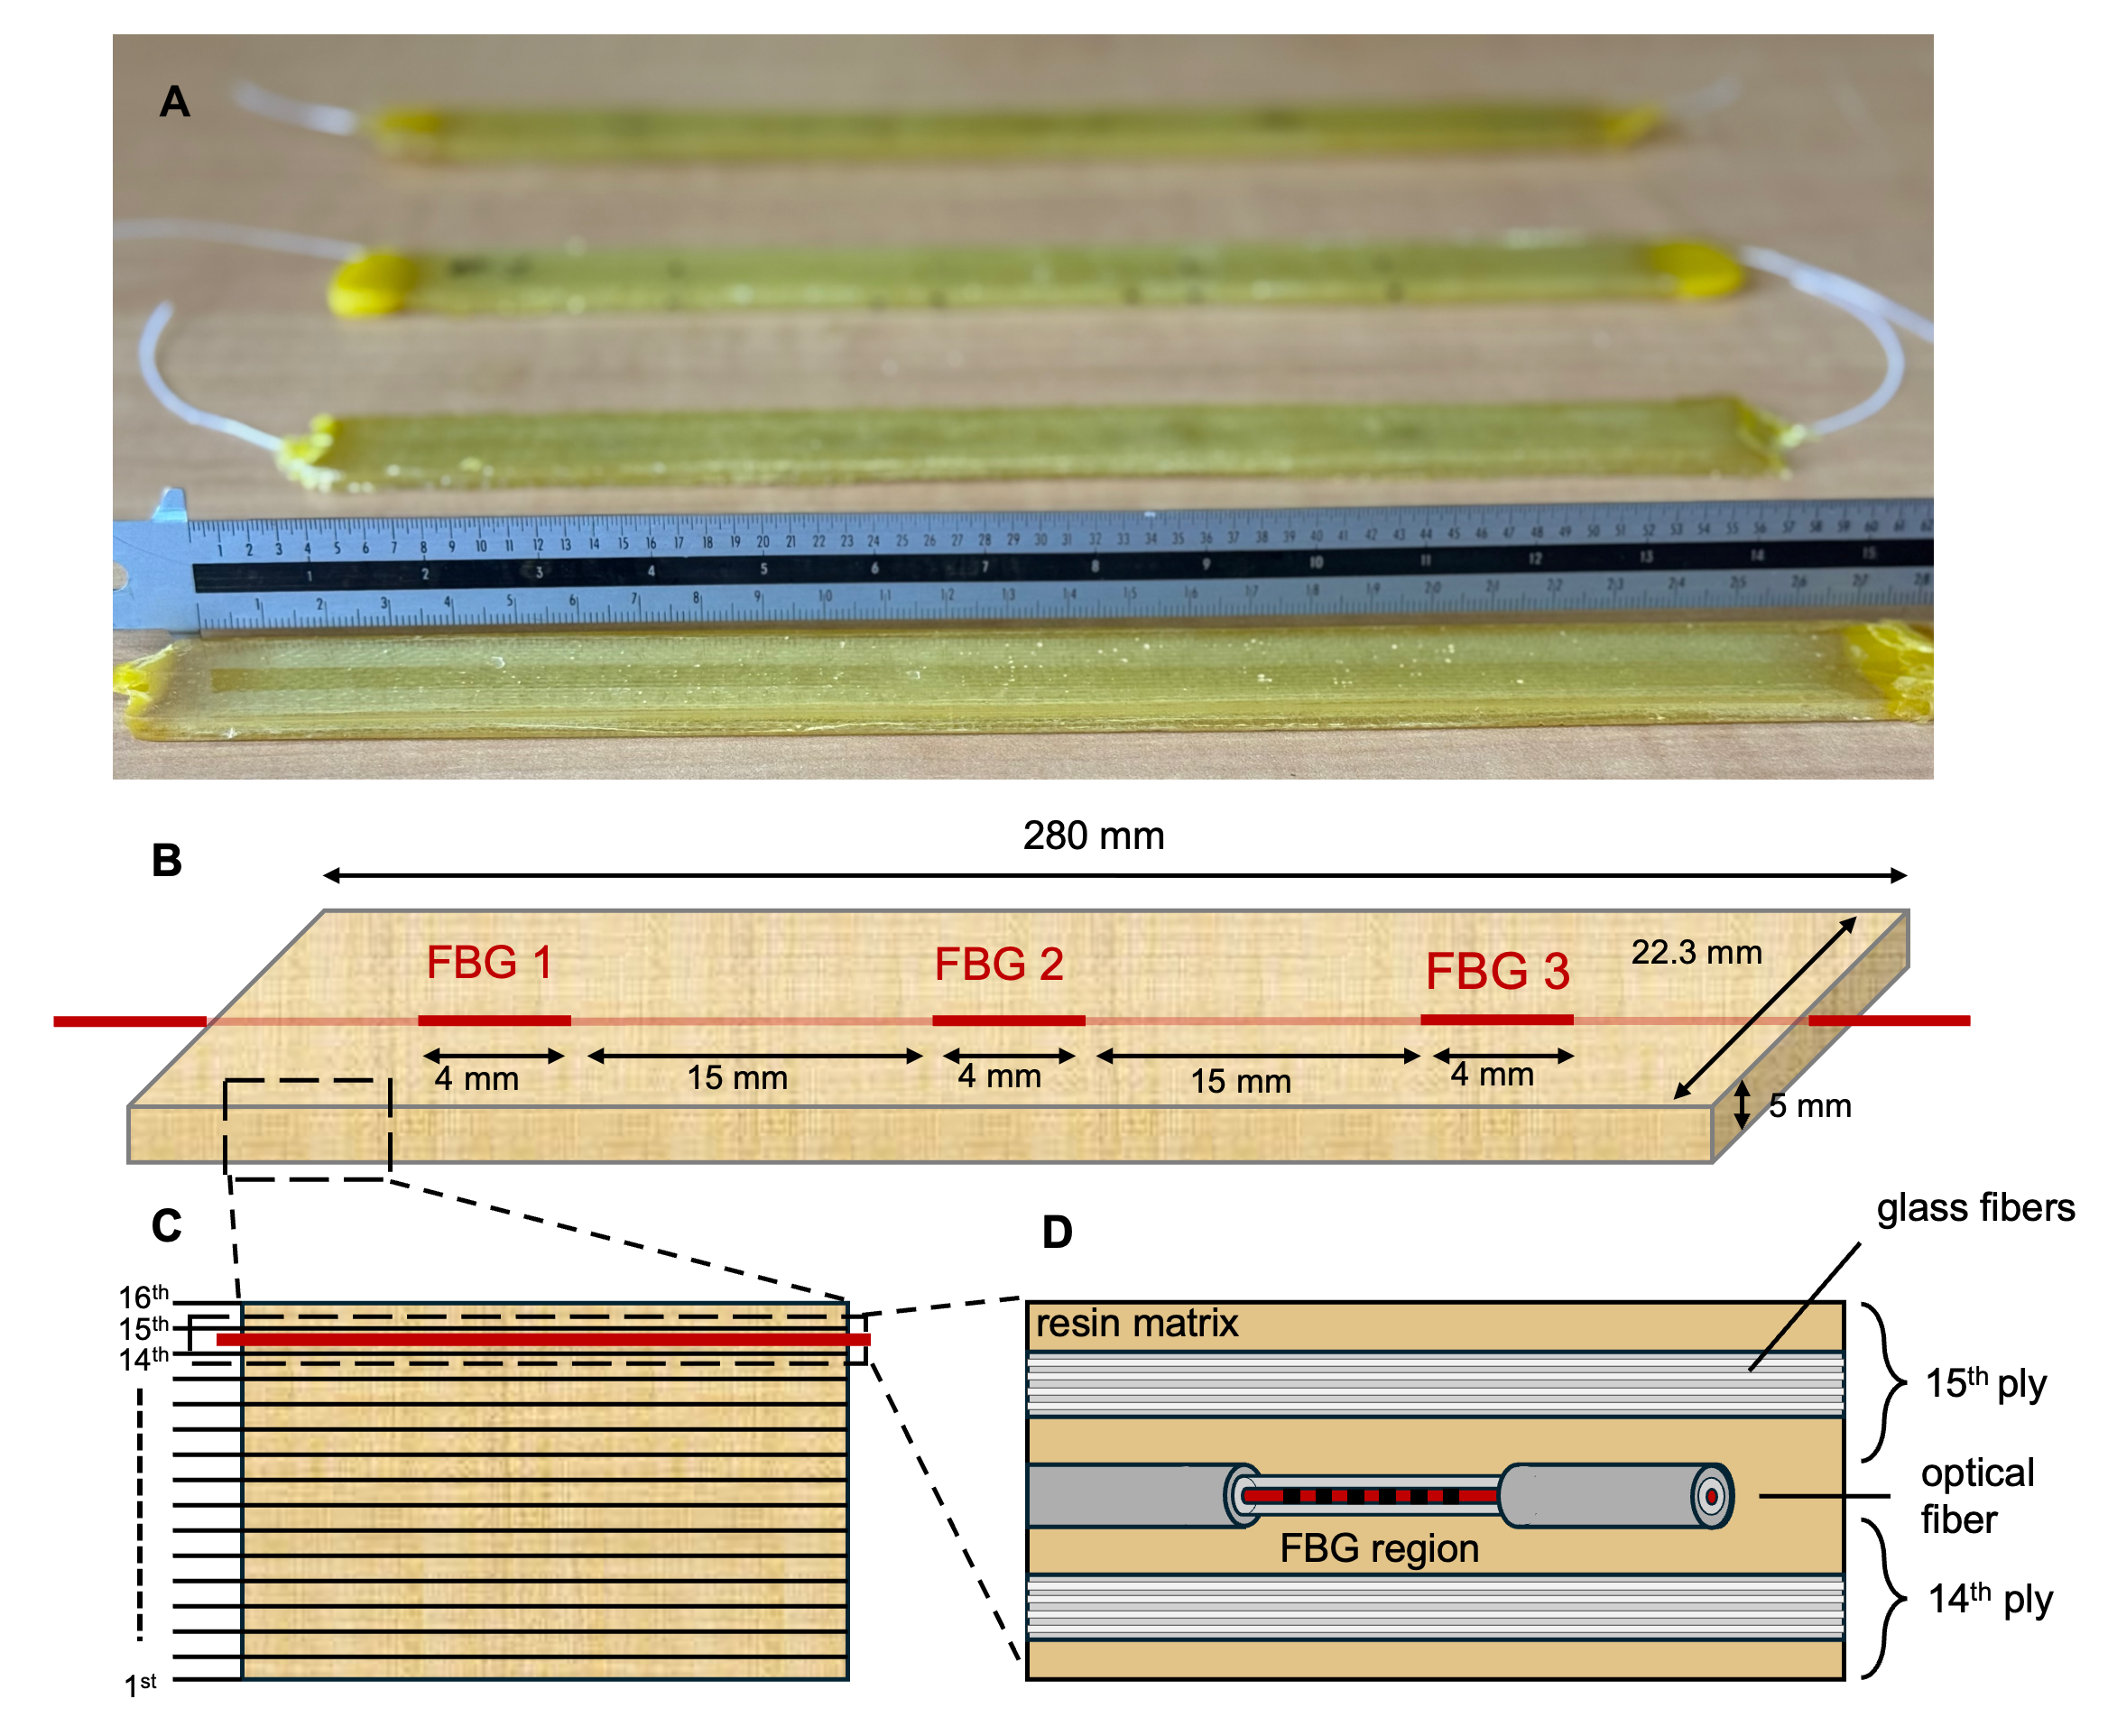
\includegraphics[width=\linewidth]{img/sketch-of-plies-together}
\caption{Fabricated composite specimens, specimen geometry, laminate layup, and local sensor embedding. Panel (a) shows representative hand-laminated glass-fiber-reinforced polymer specimens used in the three-point bending experiments, with a ruler provided for scale. Panel (b) shows the specimen geometry, nominal dimensions, and the positions of the three embedded FBGs along the optical fiber. Panel (c) shows a cross-section schematic of the 16-ply laminate, highlighting fiber placement between the 14th and 15th plies near the upper surface. Panel (d) shows a close view of this interply region, indicating the glass fiber layers, resin matrix, embedded optical fiber, and the FBG sensing region.\label{fig:composite_sample}}
\end{figure}

\subsection{Three-Point Bending Experiments}

Mechanical testing was performed with a pneumatic three-point bending system instrumented to measure applied force and crosshead displacement. Each specimen was placed on two supports separated by a prescribed span, and load was applied at midspan. The actuator force was controlled through discrete air-pressure settings. For each selected pressure level, ten consecutive loading cycles were applied before moving to the next level. This protocol produced repeated measurements within a given loading block while progressively increasing the loading level on the specimen. During each test, the bending machine recorded force, displacement, and applied pressure, while the embedded FBGs were interrogated in parallel by the BSI-108 FBG interrogator from B-Sens. The instrumented bending setup is shown in Figure~\ref{fig:bending_setup}. In the current dataset, support spans of 110, 150, 190, and 230 mm were investigated, and the nominal specimen width was 22.3 mm.

\begin{figure}[H]
\centering
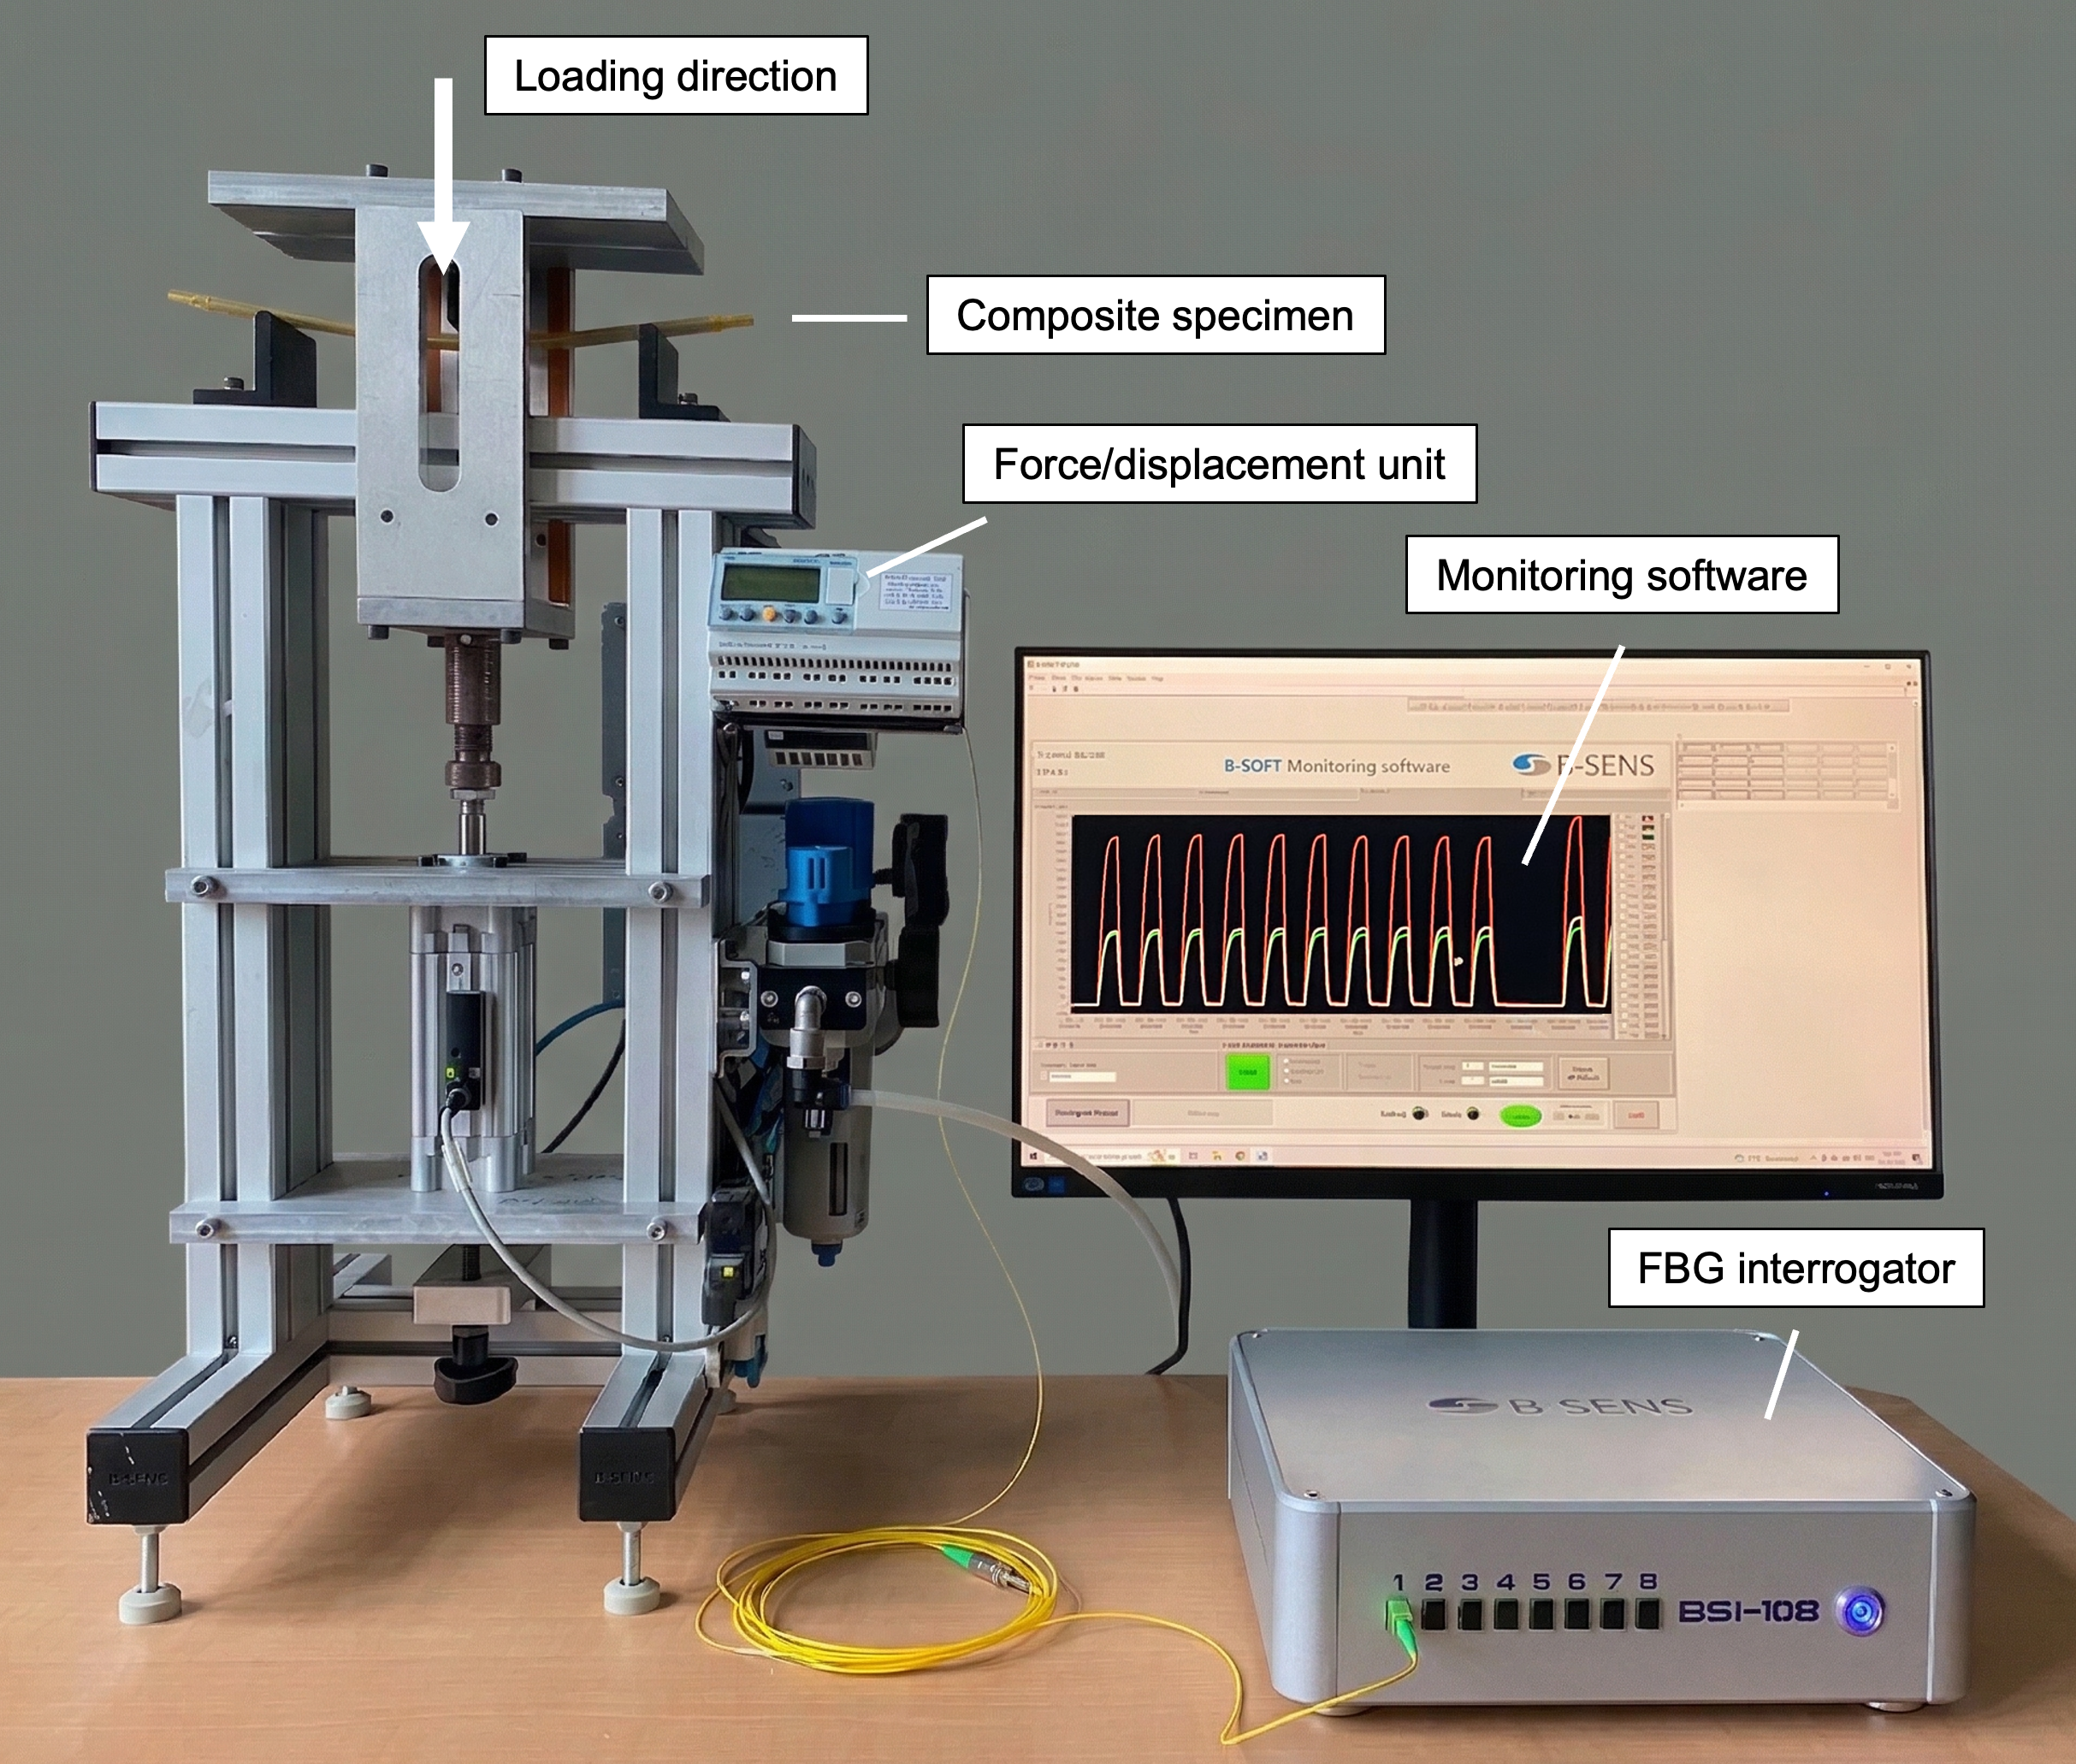
\includegraphics[width=0.72\textwidth]{img/experiment-setup-annotated}
\caption{Three-point bending measurement chain and experimental setup. The image shows the instrumented three-point bending system used in the experiments, including the loading direction, the composite specimen, the force/displacement unit, the acquisition computer, and the BSI-108 FBG interrogator.\label{fig:bending_setup}}
\end{figure}

\subsection{Elastic Calibration and Mechanics-Guided Loading Interpretation}

The mechanics-guided part of the study is anchored in the linear elastic response of a slender beam under three-point bending. Similar FBG bending studies have shown that, when embedding is well controlled, the measured wavelength shift can be interpreted consistently with beam-theory strain fields in the elastic regime \cite{gabardi2023}. For a simply supported specimen loaded at midspan, the applied force generates a bending moment
\begin{equation}
M = \frac{F L}{4},
\end{equation}
where $F$ is the applied force and $L$ is the support span. According to Euler--Bernoulli beam theory, the longitudinal stress varies linearly with the distance $y$ from the neutral axis \cite{ochsner2021},
\begin{equation}
\sigma = \frac{M y}{I},
\end{equation}
where $I$ is the second moment of area of the cross section. For the rectangular specimens considered here,
\begin{equation}
I = \frac{b h^3}{12},
\end{equation}
with $b$ the specimen width and $h$ the specimen thickness. Assuming linear elastic behavior before crack initiation, $\varepsilon = \sigma / E$, so the strain at the FBG position becomes
\begin{equation}
\varepsilon = \frac{M y_{\mathrm{FBG}}}{E I} = \frac{3 F L y_{\mathrm{FBG}}}{E b h^3},
\label{eq:euler_bernoulli_strain}
\end{equation}
where $E$ is the effective Young's modulus and $y_{\mathrm{FBG}}$ is the signed distance of the sensor from the neutral axis.

Before using loading-aware features in the learning pipeline, the elastic bending response was examined to verify that beam theory described the behavior before crack initiation. As shown in Figure~\ref{fig:calibration_plots}, panel (a), the applied force increased approximately linearly with the measured displacement over the initial loading regime of the calibration specimens. Using the measured wavelength shifts, an FBG strain sensitivity of 1.2 pm/$\mu\varepsilon$ determined from a separate calibration process, and Equation~\ref{eq:euler_bernoulli_strain}, an effective Young's modulus was estimated from pre-crack calibration data. Figure~\ref{fig:calibration_plots}, panel (b), shows that the resulting modulus values remained clustered around 18.6 GPa across the investigated force range, with limited dispersion. This supported the use of a single effective modulus of 18.6 GPa for mechanics-guided interpretation, a value consistent with reported elastic moduli for GFRP laminates and woven GFRP composites in the literature \cite{bazli2019,gao2016}.

\begin{figure}[H]
\centering
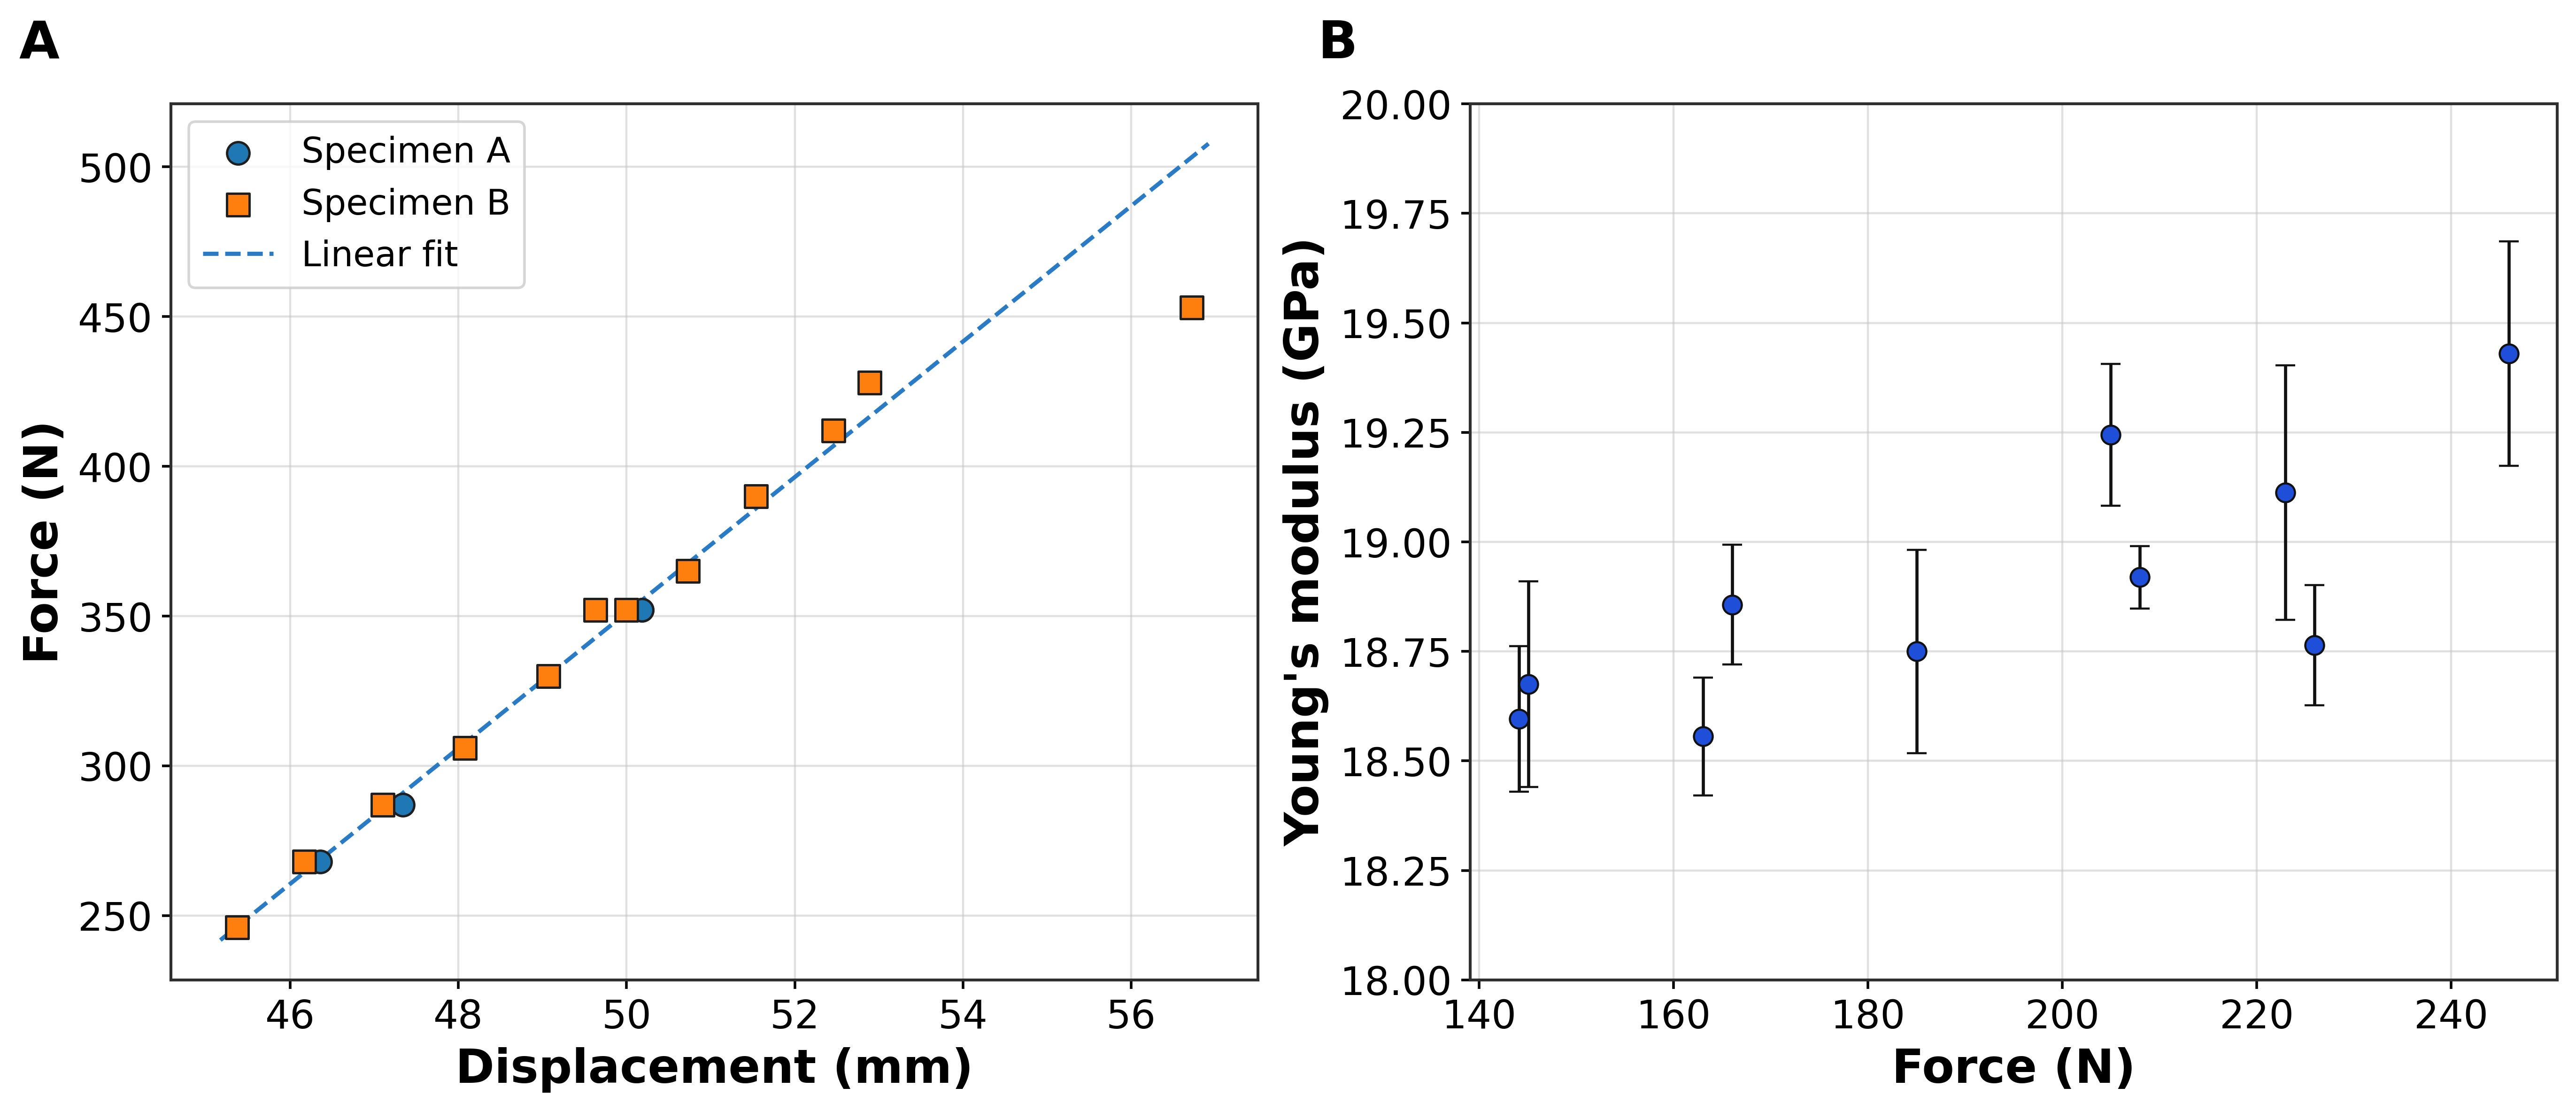
\includegraphics[width=\linewidth]{img/calibration_mechanics_combined}
\caption{Calibration of the 16-ply specimens in the elastic regime. Panel (a) shows the measured force as a function of displacement for representative specimens, together with the fitted linear trend used to identify the initial elastic regime. Panel (b) shows the effective Young's modulus estimated from calibration measurements before crack initiation using the FBG wavelength shifts and the Euler--Bernoulli bending relation.\label{fig:calibration_plots}}
\end{figure}

\subsection{Data Acquisition, Peak Alignment, and Window Construction}

The dataset was built from two synchronized sources: raw multiplexed interrogator recordings and experiment-level mechanical metadata. The FBG interrogator tracked the Bragg peak evolution of the active sensor channels over the 1510--1590 nm spectral range with sub-picometer wavelength resolution, while the bending setup recorded force, displacement, applied pressure, support span, and specimen geometry for each loading group. The learning dataset was reconstructed directly from the raw interrogator text files and the associated experiment metadata rather than from pre-aggregated summary tables. This design preserves the waveform shape of each loading response, exposes the alignment path explicitly, and retains the information needed to test whether loading context improves detection.

Each experimental run was segmented into repeated loading responses centered on interrogator peaks. Two alignment strategies were examined: a fully automatic peak search performed directly on the raw interrogator traces, and a hybrid strategy using segment-boundary hints extracted from the aligned experiment records when those hints were available and internally consistent. The hybrid strategy produced the most stable run-level classification results and was therefore used for the main experiments. After segmentation, each retained response was resampled to a fixed-length representation while preserving the synchronized target channel and companion channels from the same multiplexed acquisition. This reconstruction step was central to the study because it converted raw interrogator files into repeatable learning units tied to the mechanical loading history.

The final dataset contained 64 processed runs. For most runs, 120 peak-centered responses were retained, corresponding to 12 loading groups with 10 repetitions per group. Each response was associated with a run identifier, loading-group index, repetition index, sample indices in the original interrogator trace, its cracked or non-cracked state, and the synchronized loading metadata for the corresponding mechanical block. In addition to the raw interrogator channels, the dataset stored aligned loading traces for applied pressure, force, displacement, and an approximate elastic strain target derived from beam theory. This made it possible to derive compact sequence features from the optical response while preserving the synchronized mechanical context.

The evaluated set contained 15 crack-positive runs. The task is formulated as crack-event detection from multiplexed FBG measurements, with the cracked state interpreted at the loading-group level and propagated to the sequence windows used for learning.

Mechanical metadata were aligned to the interrogator responses at the level of repeated loading blocks. Force, displacement, pressure, support span, specimen thickness, and specimen width were assigned to each retained response through the combination of run identifier and loading-group index. These synchronized quantities were then used to derive the retained loading features and the mechanics-guided residual terms. Because responses from the same run remained temporally and mechanically correlated, all evaluation protocols were performed at run level rather than by random splitting.

Figure~\ref{fig:window_mosaic} shows this hierarchy on one sequence. Panel (a) shows the full interrogator run together with one representative loading group. Panel (b) zooms into the corresponding 10-response group and highlights responses before crack initiation and crack responses. Panels (c) and (d) then show the individual responses used to illustrate the local waveform changes observed across the multiplexed FBG channels before and after crack initiation.

\begin{figure}[H]
\centering
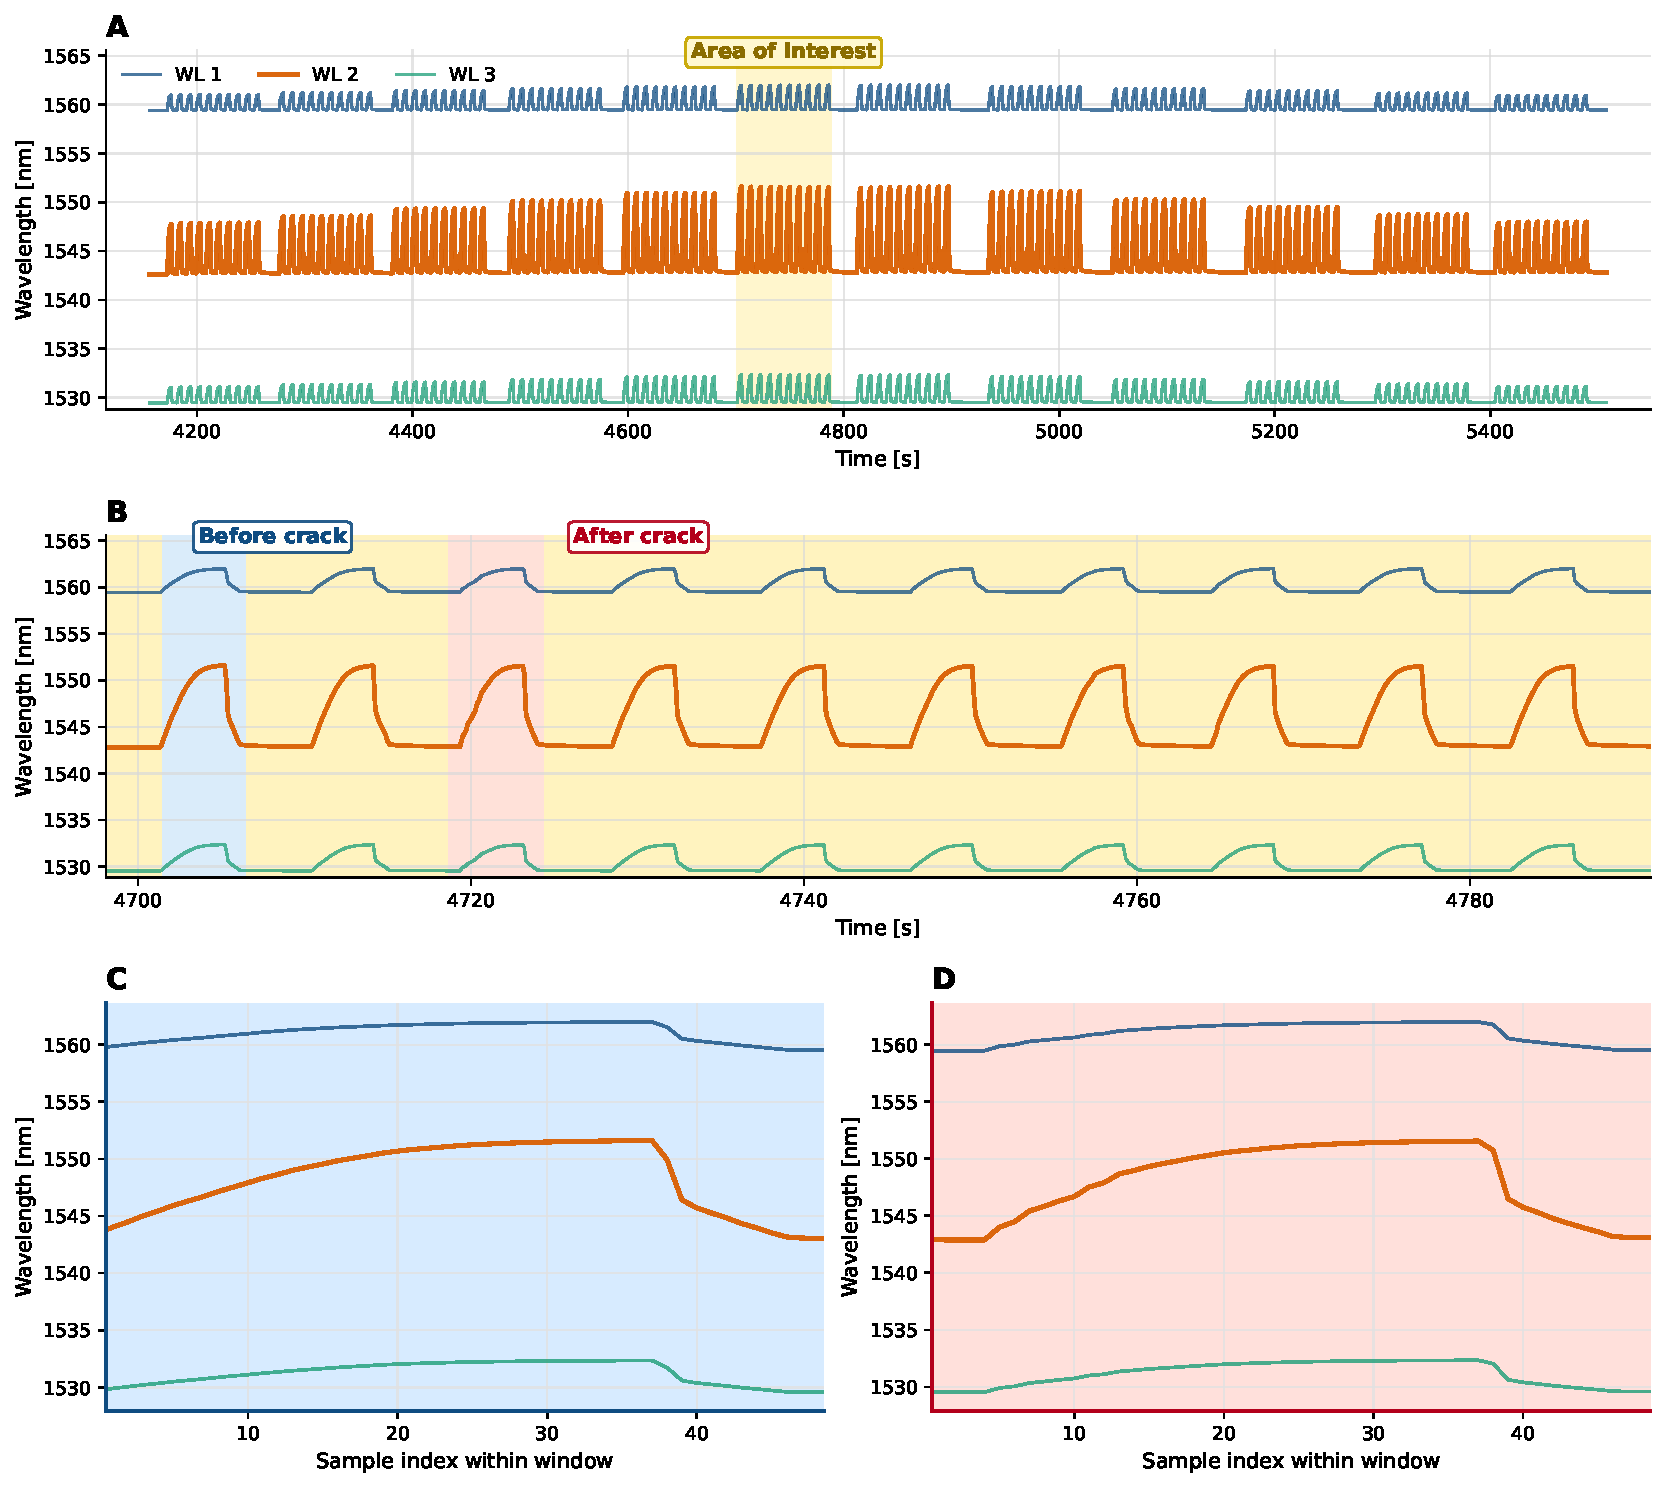
\includegraphics[width=\linewidth]{img/mosaic_time_series_before_after}
\caption{Example raw interrogator sequence and response hierarchy used for learning. Panel (a) shows the full multiplexed FBG interrogator run, with one representative loading group highlighted. Panel (b) shows the corresponding 10-response group on a shorter time scale, with responses before crack initiation and crack responses highlighted. Panels (c) and (d) show the individual responses before and after crack initiation, respectively, for the target FBG channel together with its two companion channels.\label{fig:window_mosaic}}
\end{figure}

\subsection{Sequence Representation and Selected Input Features}

The selected representation encodes each repeated peak-centered response as a compact feature vector instead of the full interrogator waveform. This representation was retained because it produced the most reproducible grouped detection result among the evaluated alternatives while keeping the mechanics contribution explicit. Thirteen features were used in the final model: the median wavelength of the target channel, the within-response standard deviation of that wavelength, a run-baseline-residualized target-channel wavelength shift, synchronized force, synchronized crosshead displacement, applied air pressure, the first-difference of the residualized wavelength shift across consecutive responses, the first-difference of the displacement signal across consecutive responses, the Euler--Bernoulli expected elastic strain, the observed strain inferred from the retained wavelength sensitivity, a normalized mechanics residual, the change of that residual relative to the run baseline, and a binary flag indicating the reduced-size specimen subgroup identified in the source filenames. These features are summarized in Table~\ref{tab:input_summary}.

\begin{table}[H]
\caption{Thirteen input features used by the selected physics-guided sequence CNN.\label{tab:input_summary}}
\begin{tabularx}{\textwidth}{p{0.24\textwidth}X}
\toprule
\textbf{Feature} & \textbf{Description} \\
\midrule
\texttt{wl2\_median} & Median wavelength of the target FBG channel within the retained peak-centered response. \\
\texttt{wl2\_std} & Standard deviation of the target-channel wavelength within the retained response. \\
\texttt{delta\_wl\_ch2} & Target-channel wavelength shift residualized relative to the run baseline. \\
\texttt{force\_N} & Synchronized applied force for the aligned loading block. \\
\texttt{displacement\_mm} & Synchronized crosshead displacement for the aligned loading block. \\
\texttt{air\_pressure\_bar} & Pneumatic loading pressure associated with the aligned loading block. \\
\texttt{delta\_wl\_rate} & First-difference of \texttt{delta\_wl\_ch2} across consecutive retained responses within the same run. \\
\texttt{delta\_disp\_rate} & First-difference of displacement across consecutive retained responses within the same run. \\
\texttt{expected\_elastic\_strain\_microstrain} & Elastic strain expected from the synchronized loading state through the Euler--Bernoulli bending relation. \\
\texttt{observed\_strain\_microstrain\_sensitivity} & Strain inferred from the measured wavelength response using the retained FBG sensitivity calibration. \\
\texttt{mechanics\_residual\_normalized} & Normalized deviation between the observed strain and the Euler--Bernoulli elastic expectation. \\
\texttt{mechanics\_residual\_change\_from\_baseline} & Change of the normalized mechanics residual relative to its run baseline. \\
\texttt{is\_small\_sample} & Binary indicator for the reduced-size specimen subgroup encoded in the source filenames. \\
\bottomrule
\end{tabularx}
\end{table}

Each learning sample comprised 30 consecutive retained responses from the same run, with stride 1. The label attached to each 30-response sequence was the maximum of the crack-event labels already present within that sequence and the label observed at a prediction horizon of 5 responses beyond the sequence end. This rule preserved sensitivity to transitions that emerged near the end of a local response history while keeping the sequence definition fixed across runs. Feature normalization was fitted on the training split only within each validation fold.

\subsection{Selected Simple Sequence CNN}

The retained classifier is a compact one-dimensional CNN operating on a $30\times13$ input array, where the 30 rows correspond to ordered retained responses and the 13 columns correspond to the synchronized feature set described above. During inference, the feature dimension is treated as the channel dimension and the sequence order is treated as the temporal dimension. The network uses three temporal convolution layers with 32, 64, and 128 channels, all with kernel size 12 and padding 6, each followed by a rectified linear unit activation. Adaptive average pooling then compresses the temporal representation to a single 128-dimensional embedding, which is passed to a classifier head composed of a 64-unit fully connected layer, rectified linear unit activation, dropout of 0.2, and a final linear output layer producing one crack-event logit.

This architecture was selected because it keeps the modeling pipeline simple while still allowing the network to learn short-range temporal motifs across consecutive loading responses. Figure~\ref{fig:cnn_architecture} shows the retained CNN used for the main result.

\begin{figure}[H]
\centering
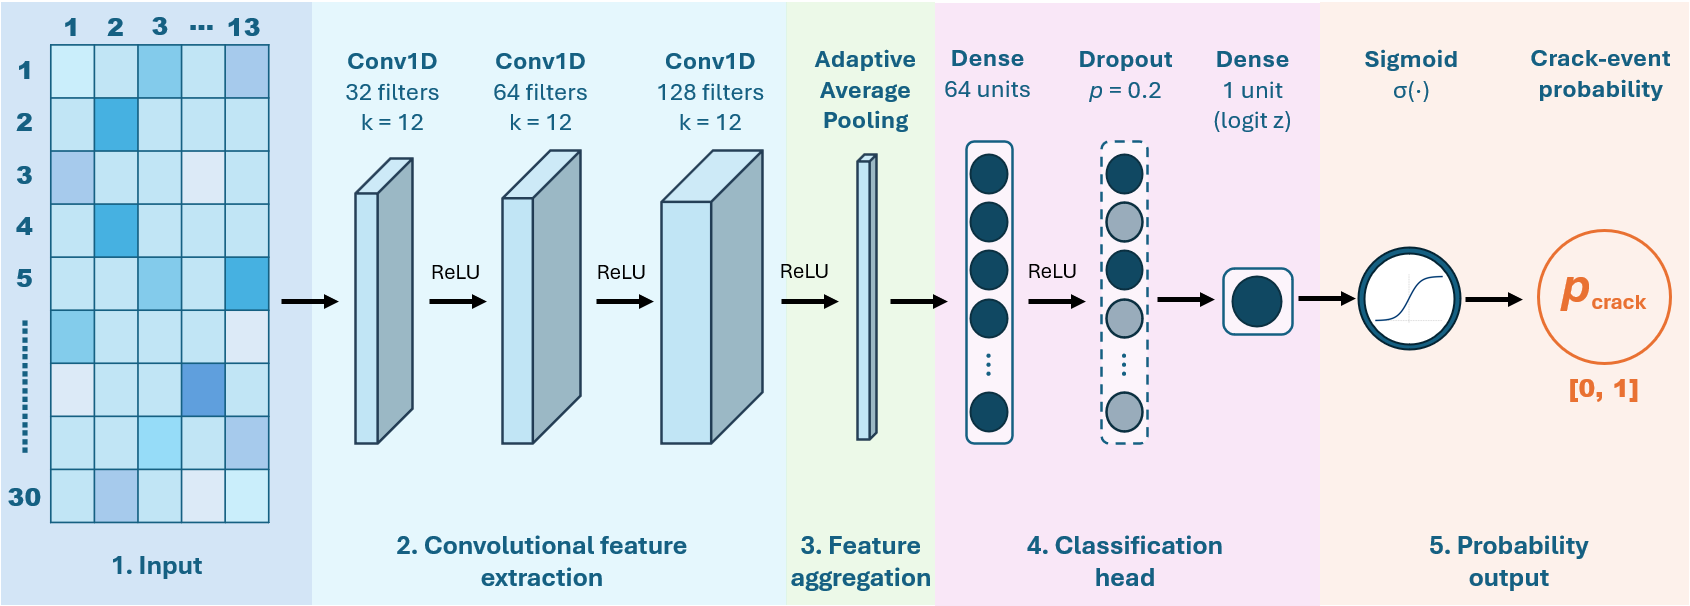
\includegraphics[width=\linewidth]{img/cnn-simplified}
\caption{Compact one-dimensional sequence CNN retained for the main result. Each input sample is a $30\times13$ feature tensor built from 30 consecutive peak-centered responses and 13 synchronized optical, loading, and mechanics-guided features. The network applies three temporal convolution layers with 32, 64, and 128 filters, all with kernel size 12, each followed by rectified linear unit activation, then adaptive average pooling, a 64-unit dense layer with rectified linear unit activation, dropout with probability 0.2, and a sigmoid output for crack-event probability estimation.\label{fig:cnn_architecture}}
\end{figure}

\subsection{Training, Model Selection, and Evaluation}

This study uses grouped evaluation because neighboring retained responses from the same run are highly correlated. The main protocol therefore uses leave-one-run-out validation, implemented as leave-one-group-out cross-validation with the run identifier as grouping variable. In this setting, each held-out fold corresponds to an unseen experimental run, the primary predictions are generated at the 30-response window level, and run-level predictions are obtained by aggregating the sequence predictions within that run.

The selected operating point used the reconstructed aligned dataset described above. Training used weighted binary cross-entropy to account for class imbalance, a fixed random seed, batch size 128, Adam optimization with learning rate $10^{-3}$ and weight decay $10^{-4}$, a maximum of 8 epochs, and early stopping with patience 3 on the inner validation split. The retained evaluation set yielded 5204 valid sequence windows, including 1045 positive windows under the fixed window target used in the main experiment. This configuration preserved a compact training procedure while providing stable grouped generalization across held-out experiments.

At the end of each fold, validation probabilities were used to select the decision threshold. The retained physics-guided operating point uses a fixed threshold of 0.45. No additional post-hoc physics filter was applied to the predictions reported here. Instead, the mechanics contribution is already embedded in the input tensor through the expected elastic strain and residual-deviation descriptors derived from the synchronized loading history.

Figure~\ref{fig:residual_confirmation} illustrates this mechanics-guided signal on a representative crack-positive sequence from the retained dataset. The plotted residual deviation is computed from the difference between the observed strain inferred from the target FBG response and the Euler--Bernoulli elastic expectation under the synchronized loading history. The marked jump at the crack-associated stage is representative of the residual behavior summarized by the mechanics-aware descriptors used in the CNN input tensor.

\begin{figure}[H]
\centering
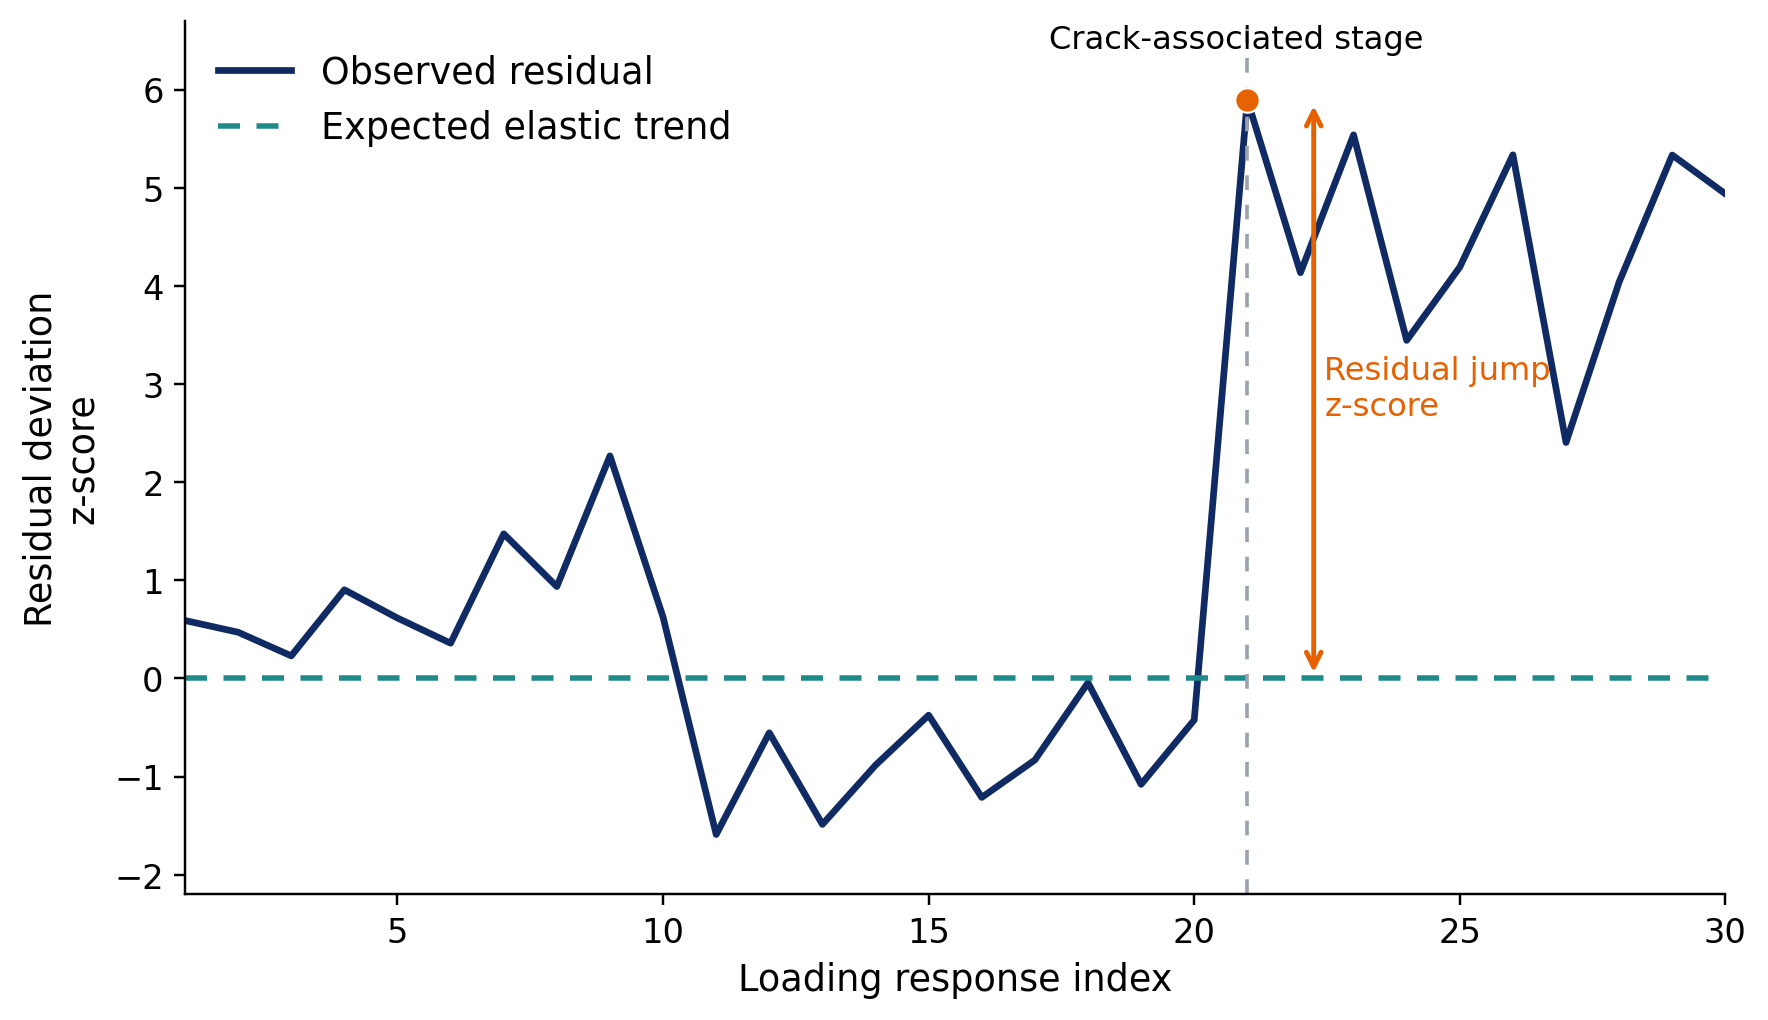
\includegraphics[width=0.82\linewidth]{img/residual_confirmation_real_plot}
\caption{Representative residual load--wavelength deviation trace from the retained dataset. The solid curve shows the standardized observed residual deviation over a 30-response sequence, while the dashed horizontal reference indicates the expected elastic trend. The highlighted jump at the crack-associated stage illustrates the mechanics-guided discrepancy signal from which the residual input descriptors were derived.\label{fig:residual_confirmation}}
\end{figure}

Window-level precision, recall, $F_1$, and balanced accuracy are reported first because they reflect the local crack-event discrimination learned by the model under run-grouped validation. Run-level aggregation metrics are then reported as specimen-scale screening indicators derived from the same window predictions.

\subsection{Statistical Reporting and Validation Scope}

Because neighboring responses within the same experiment are not independent, all uncertainty estimates were computed by bootstrap resampling at run level. In addition to the point estimates reported for the main operating point, 95\% confidence intervals were estimated by nonparametric bootstrap resampling of the 64 evaluated runs with replacement over 5000 iterations. For window-level metrics, each resampled run contributed all of its corresponding windows; for run-level metrics, each resampled run contributed a single aggregated label. This provides uncertainty bands tied to the independent experimental units rather than to the much larger number of overlapping response windows.

No separate external cohort acquired in another fabrication campaign was available for a fully independent external validation. The present work therefore emphasizes grouped within-campaign validation, run-bootstrap confidence intervals, and explicit separation between local window-level discrimination and specimen-level aggregation.

\section{Results}

\subsection{Window-Level and Run-Level Detection Performance}

The main evaluation was performed with strict leave-one-run-out validation on the retained dataset. Table~\ref{tab:overall_performance} reports the window-level metrics of the retained physics-guided CNN together with the corresponding run-level aggregation obtained from the same predictions.

\begin{table}[H]
\caption{Main results for the retained physics-guided CNN operating point on the retained dataset.\label{tab:overall_performance}}
\begin{tabularx}{\textwidth}{XCCCC}
\toprule
\textbf{Evaluation Level} & \textbf{Precision} & \textbf{Recall} & \textbf{$F_1$} & \textbf{Balanced Accuracy} \\
\midrule
Window level & 0.900 & 0.910 & 0.905 & 0.942 \\
Run level & 0.833 & 1.000 & 0.909 & 0.969 \\
\bottomrule
\end{tabularx}
\end{table}

Bootstrap resampling over the 64 evaluated runs showed that the main result remained stable under grouped uncertainty estimation. At window level, the retained operating point yielded an $F_1$ of 0.905 with a 95\% bootstrap confidence interval of 0.787--0.978, while the balanced accuracy was 0.942 with a 95\% interval of 0.871--0.989. After aggregation to run level, the $F_1$ was 0.909 with a 95\% bootstrap confidence interval of 0.769--1.000, and the balanced accuracy was 0.969 with a 95\% interval of 0.930--1.000. These intervals support the stability of the physics-guided operating point within the present campaign.

\subsection{Confusion-Matrix View of the Retained Operating Point}

The confusion matrices of the retained operating point are shown in Figure~\ref{fig:confusion_matrices}. At window level, the model produced 4054 true negatives, 105 false positives, 95 false negatives, and 950 true positives. This distribution is consistent with the balanced precision and recall reported in Table~\ref{tab:overall_performance}, showing that the compact CNN separates crack-associated windows effectively while keeping both error types limited.

At run level, aggregation of the same window predictions yielded 46 true-negative runs, 3 false-positive runs, 0 false-negative runs, and 15 true-positive runs. This aggregation preserved perfect sensitivity to crack-positive runs while limiting overprediction to three negative runs in the present campaign.

\begin{figure}[H]
\centering
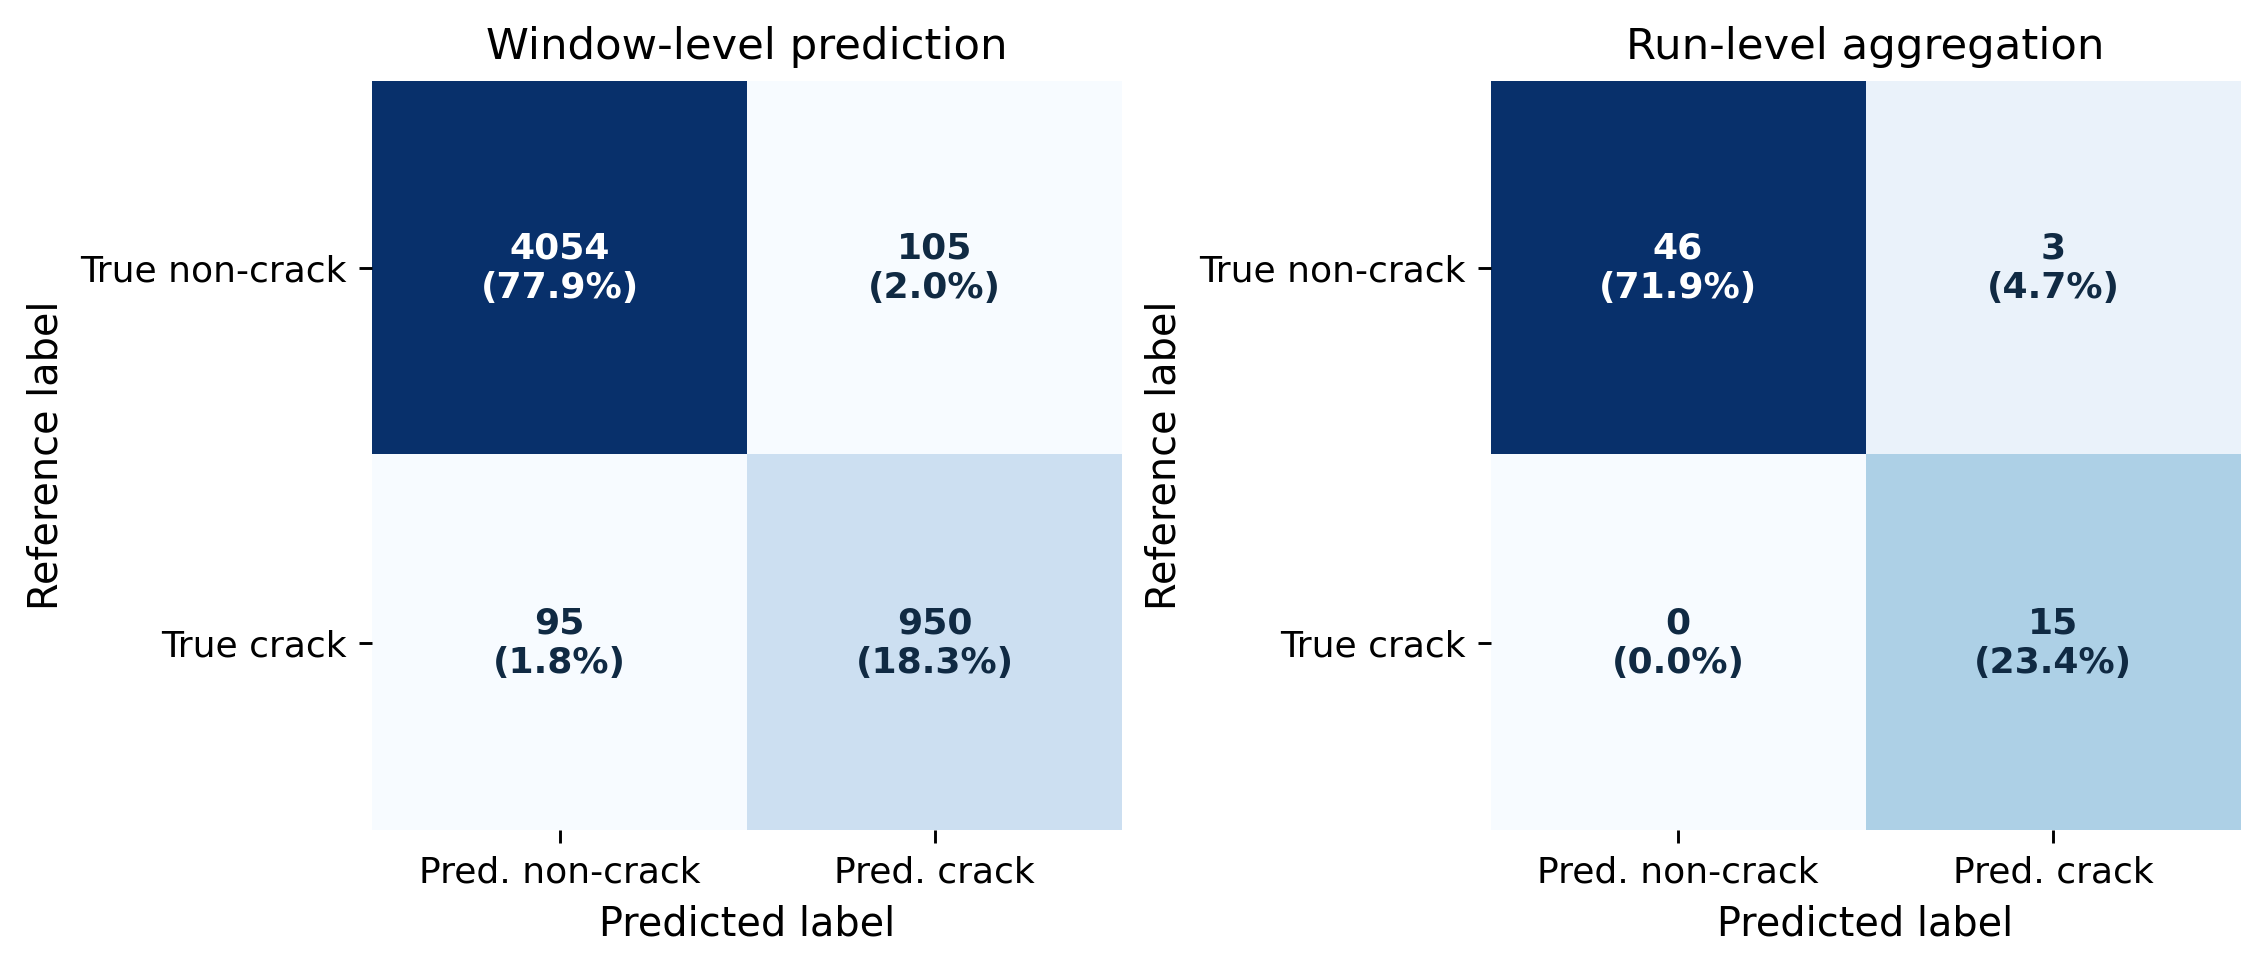
\includegraphics[width=\linewidth]{img/confusion_matrices_physics_guided}
\caption{Confusion matrices for the retained physics-guided CNN operating point. The left panel reports the primary window-level predictions under strict leave-one-run-out validation. The right panel reports the corresponding run-level aggregation obtained by marking a run positive when at least one of its windows crosses the retained threshold.\label{fig:confusion_matrices}}
\end{figure}

\subsection{Mechanics-Guided Interpretation of the Detection Pipeline}

The mechanics-guided contribution of the pipeline appears directly in the retained feature space. Euler--Bernoulli theory provides the elastic strain expectation used to relate applied force, specimen geometry, and the healthy loading response. The synchronized force and displacement variables anchor this expectation to the actual mechanical state of each loading block. The residual descriptors then quantify departures from the expected elastic behavior and expose precisely the kind of load--wavelength inconsistency that accompanies crack-associated events. This combination explains why a compact CNN can remain simple while still reaching strong local and aggregated detection performance.

\section{Discussion}

These results show that crack-event detection is feasible from short peak-aligned responses of multiplexed FBG interrogator data when synchronized loading metadata and mechanics-guided residual descriptors are incorporated into the pipeline. The retained operating point reached balanced window-level detection while also preserving perfect run-level recall on the present dataset. This is important because it shows that useful specimen-level damage information can be extracted from compact multiplexed FBG measurements with a method that remains both interpretable and computationally light.

The results also show that metric choice matters. Window-level scores capture the local discrimination learned by the model, whereas run-level scores capture the specimen-scale screening behavior after aggregation. Reporting both views is therefore useful in the present SHM setting: the first documents how well short loading histories are classified, and the second documents whether an unseen experimental run is flagged correctly.

Mechanics plays a practical role in the present study by structuring the detection pipeline around synchronized loading information. Force and displacement traces, expected elastic strain, and residualized load--wavelength features provide structural constraints that make the CNN sensitive to departures from healthy bending behavior rather than to wavelength variation alone. This supports the broader idea that structural priors can strengthen learning from sparse optical measurements when the sensing configuration does not provide rich spatial information.

The retained architecture is deliberately compact. Rather than relying on a heavy network, the present framework obtains its performance from the joint use of synchronized optical and mechanical descriptors, strict grouped evaluation, and a sequence model that is easy to reproduce. This simplicity is an advantage for reproducibility and makes the method straightforward to transfer to future experimental campaigns with richer sensor layouts or larger cohorts.

The added uncertainty analysis sharpens the interpretation of the reported scores. Because the bootstrap resampling was performed over runs rather than over windows, the confidence intervals are tied to the independent experimental units of the campaign. The resulting intervals confirm that the retained operating point is not an artifact of pooled window counting.

\section{Conclusions}

This study demonstrates that a compact CNN, combined with Euler--Bernoulli-guided strain interpretation, can detect crack-associated events effectively from multiplexed FBG interrogator measurements. On strict leave-one-run-out evaluation, the retained physics-guided operating point reached window-level precision of 0.900, recall of 0.910, $F_1$ of 0.905, and balanced accuracy of 0.942, while the corresponding run-level aggregation reached precision of 0.833, recall of 1.000, $F_1$ of 0.909, and balanced accuracy of 0.969. The resulting framework is simple, physically grounded, and well suited to crack-event screening in composite SHM experiments.

\authorcontributions{Conceptualization, A.U. and C.C.; methodology, A.U., A.G. and C.C.; software, A.U.; validation, A.U. and A.G.; formal analysis, A.U.; investigation, A.U., E.N., T.T. and K.C.; resources, C.C. and K.Y.; data curation, A.U., E.N. and T.T.; writing---original draft preparation, A.U. and C.C.; writing---review and editing, A.U., A.G., E.N., T.T., K.Y., K.C. and C.C.; visualization, A.U.; supervision, A.G., K.Y. and C.C.; funding acquisition, C.C. All authors have read and agreed to the published version of the manuscript.}

\funding{This work was supported by the Walloon Region of Belgium through the Interreg VI France--Wallonie--Vlaanderen program, co-funded by the European Union, under the SALOME project (No. 0100240). This work was also supported by the WEL Research Institute and the Fonds de la Recherche Scientifique (F.R.S.--FNRS).}

\institutionalreview{Not applicable.}

\informedconsent{Not applicable.}

\dataavailability{The data supporting the reported results are available from the corresponding author upon reasonable request.}

\acknowledgments{The authors thank Mariel David for assistance during the manufacturing of the composite specimens. The authors also thank Damien Kinet from B-SENS for assistance with the operation of the three-point bending system.}

\conflictsofinterest{The authors declare no conflicts of interest. The funders had no role in the design of the study; in the collection, analyses, or interpretation of data; in the writing of the manuscript; or in the decision to publish the results.}

\abbreviations{Abbreviations}{
\noindent
\begin{tabular}{@{}ll}
CNN & Convolutional neural network\\
DFOS & Distributed fiber optic sensing\\
FBG & Fiber Bragg grating\\
GFRP & Glass-fiber-reinforced polymer\\
LOOCV & Leave-one-out cross-validation at run level\\
SHM & Structural health monitoring
\end{tabular}
}

\begin{adjustwidth}{-\extralength}{0cm}
\reftitle{References}
\bibliography{sample}
\end{adjustwidth}

\end{document}
